\documentclass[12pt,a4paper]{article}
\usepackage[brazil]{babel} 
%Não necessário com XeLaTeX
%\usepackage[utf8]{inputenc}
\usepackage{graphicx}
\graphicspath{{./img/}}
\usepackage{amsmath}
\usepackage{float}
\usepackage{listingsutf8}
\usepackage{styles/c++}

\title{Relatório da Prática 6}
\author{Vítor Barbosa}
\date{\today}

\begin{document}
\maketitle
\section{Introdução}
Essa prática é uma introdução às Threads. Faremos 3 programas: um exemplo de threads em C++ usando a biblioteca padrão; um exemplo com a API do Windows (Win32); finalmente, um aplicativo com interface gráfica (GUI).
\section{Código}
\subsection{Threads com a Standard Libary}
O C++ conta, desde a versão C++11 com suporte nativo à threads pela \emph{std::thread}. Na opinião do autor, a std::thread possui uma API muito mais clara e simples que versão Win32.

Contudo, é interessante notar que aparentemente não há um método na biblioteca padrão para forçar o término de uma única thread, o que pode ser feito com Win32.

Nosso programa conta com uma classe BabyThread que implementa uma thread de exemplo, além do arquivo main que instancia várias BabyThreads com tempos de execução aleatórios.

\subsubsection*{babythread.h}
\lstinputlisting[language=C++,style=c++]{../Aula6_threads_console/babythread.h}
\subsubsection*{babythread.cpp}
\lstinputlisting[language=C++,style=c++]{../Aula6_threads_console/babythread.cpp}
\subsubsection*{main.cpp}
\lstinputlisting[language=C++,style=c++]{../Aula6_threads_console/main.cpp}

\subsection{Threads com a Api do Windows}
O código aqui foi provido pelo professor. Ele instancia uma thread que executa e periodicamente exibe um caractere . na tela por 10 segundos.
\\
\lstinputlisting[language=C,style=c++]{../Aula6_thread_winapi/main.cpp}

\subsection{Threads com Interface Gráfica}
O programa cria 2 threads, que podem ser pausadas, reativadas ou terminadas. Cada thread retorna um texto a cada 3 segundos de sua execução.
Primeiro, foi criado o formulário da janela como usual. Ele pode ser visto na figura \ref{form}.
\begin{figure}[H]
\centering
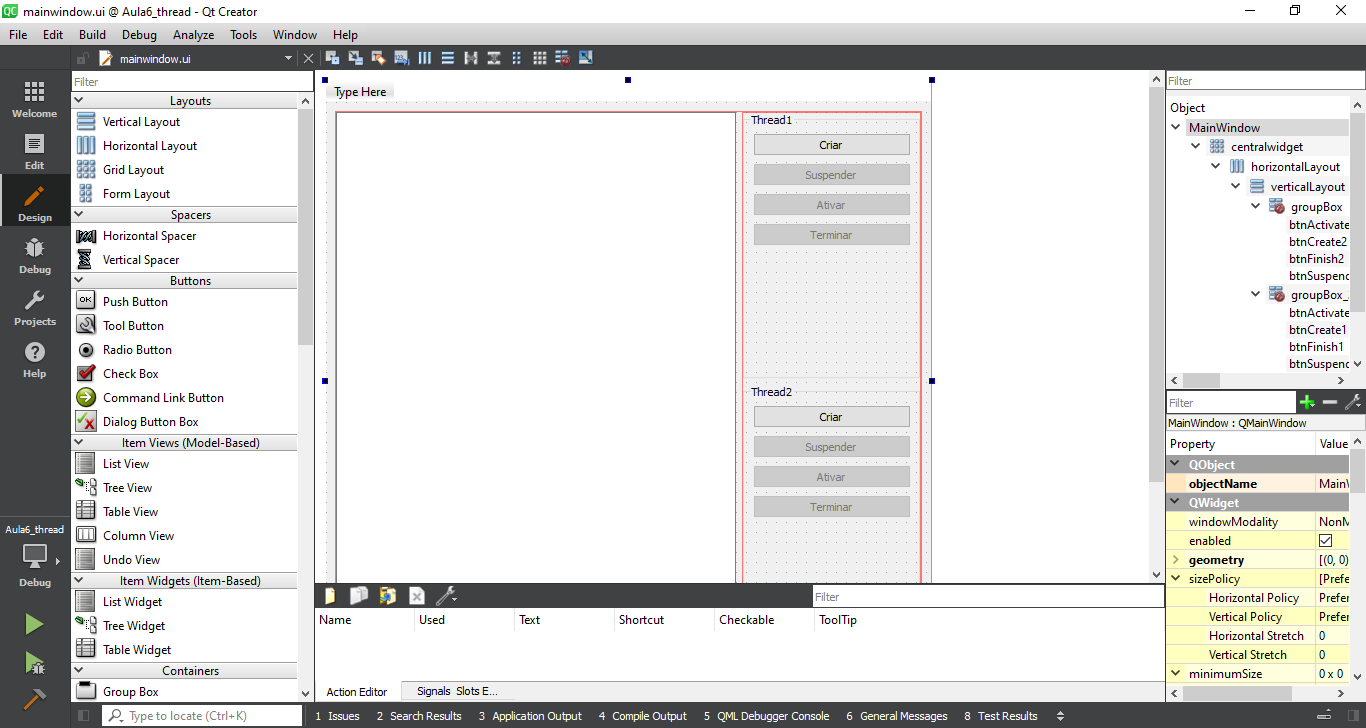
\includegraphics[width=\textwidth]{thread_form}
\caption{Criação da Janela}
\label{form}
\end{figure}
O código fonte ficou dividido entre as classes MainWindow e TextThread, além do arquivo main.
\subsubsection*{textthread.h}
\lstinputlisting[language=C,style=c++]{../Aula6_thread/textthread.h}
\subsubsection*{textthread.cpp}
\lstinputlisting[language=C,style=c++]{../Aula6_thread/textthread.cpp}
\subsubsection*{mainwindow.h}
\lstinputlisting[language=C,style=c++]{../Aula6_thread/mainwindow.h}
\subsubsection*{mainwindow.cpp}
\lstinputlisting[language=C,style=c++]{../Aula6_thread/mainwindow.cpp}
\subsubsection*{main.cpp}
Código gerado pelo Qt Creator, igual ao das práticas anteriores.
\section{Resultados}
\subsection*{Programa com a Standard Libray}
Veja na figura \ref{test_std} que 20 threads são criadas e retornam em tempos aleatórios.
\begin{figure}[H]
\centering
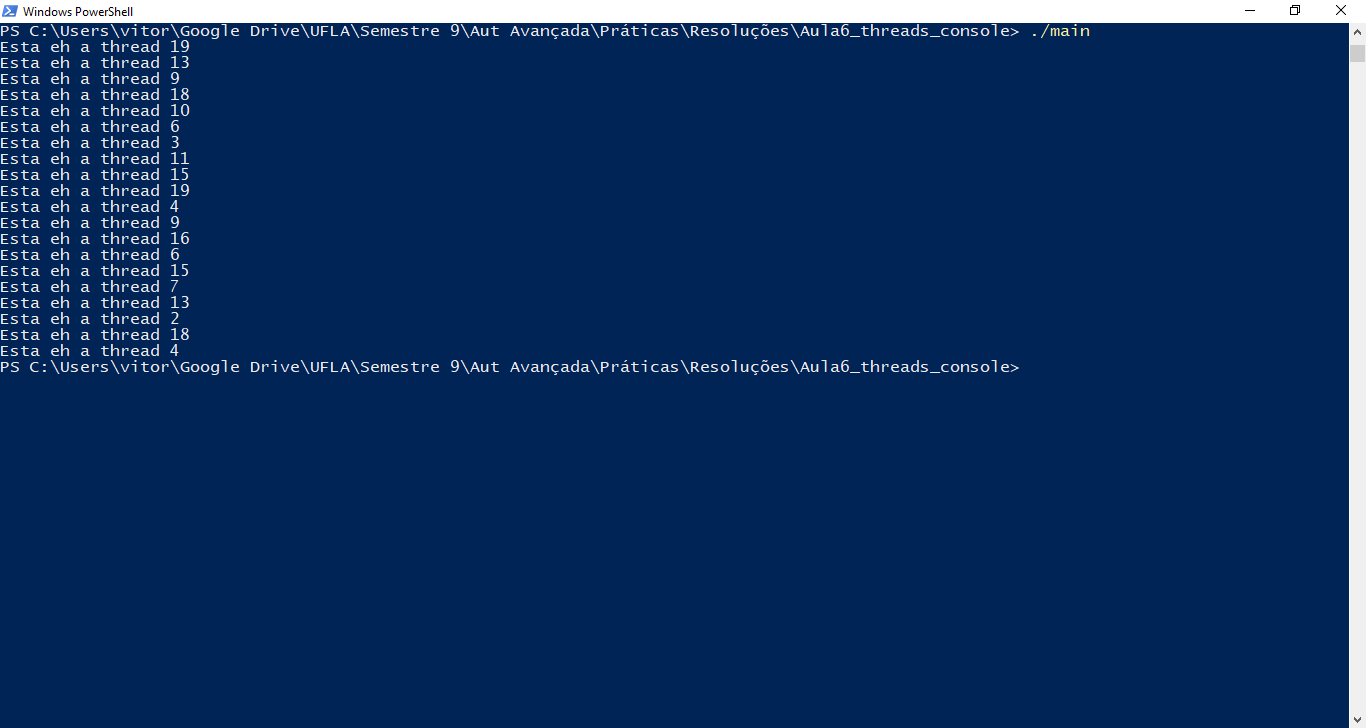
\includegraphics[width=\textwidth]{thread_std}
\caption{Teste do Programa com StdLib}
\label{test_std}
\end{figure}
\subsection*{Programa com a Api do Windows}
Veja na figura \ref{test_win32} que uma thread é criada e executada por 10s, então é forçosamente terminada. No início do console há também a saída do compilador CLang.
\begin{figure}[H]
\centering
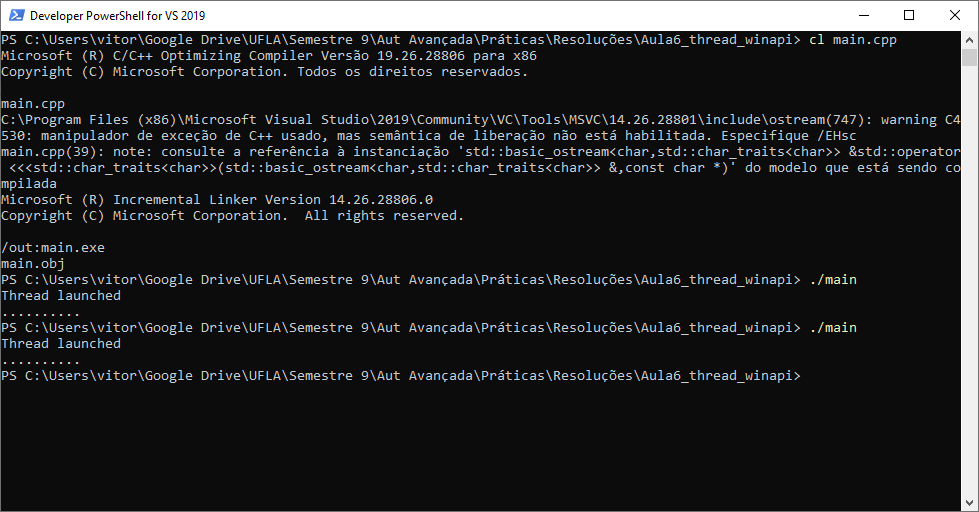
\includegraphics[width=\textwidth]{thread_winapi}
\caption{Teste do Programa com Win32}
\label{test_win32}
\end{figure}
\subsection*{Programa com o Qt}
No teste do programa com GUI, são criadas duas threads, e seu texto é exibido a cada atualização (de 3 em 3 segundos) na tela, como mostra a figura \ref{test_qt1}.

Na figura \ref{test_qt2}, a thread 1 é terminada e a thread 2 é suspensa após algum tempo.
\begin{figure}[h]
\centering
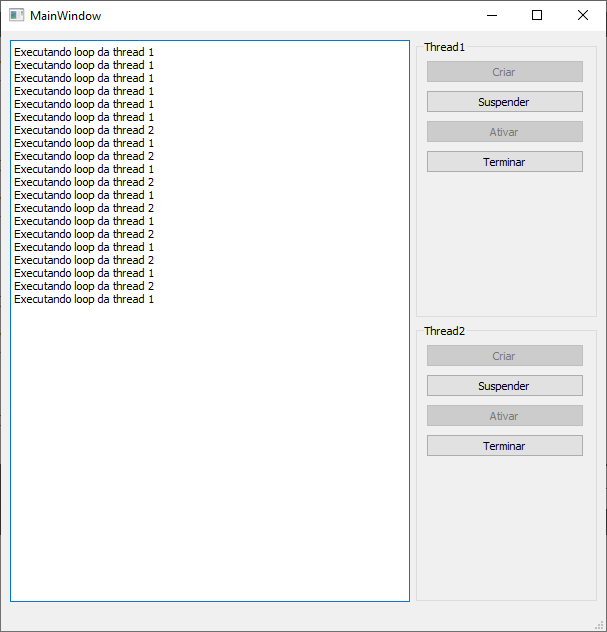
\includegraphics[width=\textwidth]{thread_test1}
\caption{Teste 1 do Programa com Qt}
\label{test_qt1}
\end{figure}
\begin{figure}[h]
\centering
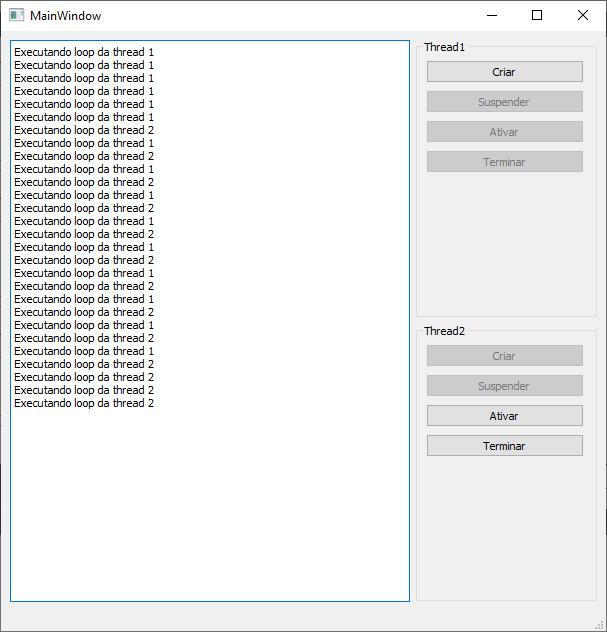
\includegraphics[width=\textwidth]{thread_test2}
\caption{Teste 2 do Programa com Qt}
\label{test_qt2}
\end{figure}
\end{document}